\documentclass[12pt,parskip=full]{article}
\usepackage{lmodern}
\usepackage{amsmath}
\usepackage[left=1.0in,right=1.0in,top=1.0in,bottom=1.0in]{geometry}
\geometry{letterpaper}
\usepackage{graphicx}
\usepackage{caption}
\usepackage{subcaption}
\usepackage{longtable}
\usepackage{float}
\usepackage{wrapfig}
\usepackage{soul}
\usepackage{textcomp}
\usepackage{marvosym}
\usepackage{wasysym}
\usepackage{latexsym}
\usepackage{amssymb}
\usepackage{apacite}
\usepackage{tabu}
\usepackage[svgnames]{xcolor}
\usepackage{tikz}
\usepackage[linktoc=all]{hyperref}
\usepackage{cleveref}
\usepackage{listings}
\usepackage{setspace}
\usepackage{parskip}
\usepackage{array}
\usepackage{apacite}
\usepackage{natbib}
\usepackage{multicol}
\usepackage{subcaption}
\usetikzlibrary{arrows}

\pgfdeclarelayer{edgelayer}
\pgfdeclarelayer{nodelayer}
\pgfsetlayers{edgelayer,nodelayer,main}

\tikzstyle{none}=[inner sep=0pt]
\tikzstyle{waypt}=[circle,fill=Black,draw=Black,scale=0.4]
\tikzstyle{Helobody}=[circle,fill=White,draw=Black,scale=4.0]
\tikzstyle{Tailrotor}=[circle,fill=White,draw=Black,scale=1.0]
\tikzstyle{ForceVector}=[->,draw=Indigo,fill=Indigo]
\tikzstyle{Coordinate}=[->,draw=Red,fill=Red,fill opacity=1.0]
\tikzstyle{angle}=[->]
\tikzstyle{MeasureMark}=[|-|]
\newlength{\imagewidth}
\newlength{\imagescale}

\setlength{\parskip}{11pt}
%\setlength{\parindent}{15pt}
\usepackage{bookmark}
\makeatletter
\renewcommand\@seccntformat[1]{}
\makeatother

\lstset
{
    language=Matlab,
    keywords={break,case,catch,continue,else,elseif,end,for,function,
        global,if,otherwise,persistent,return,switch,try,while},
    basicstyle=\ttfamily,
    keywordstyle=\color{blue},
    commentstyle=\color{ForestGreen},
    stringstyle=\color{purple},
    numbers=left,
    numberstyle=\tiny\color{gray},
    stepnumber=1,
    numbersep=10pt,
    backgroundcolor=\color{white},
    tabsize=4,
    showspaces=false,
    showstringspaces=false
}

\renewcommand{\thesection}{\arabic{section}}

\renewcommand{\thesubsection}{\thesection\alph{subsection}}
\renewcommand{\theequation}{\thesubsection\arabic{equation}}

\numberwithin{subsection}{section}

\begin{document}
	\vspace{-2ex}
	\title{Report 2: So Many Derivatives\vspace{-3.5ex}}
	\author{Rob Rau\vspace{-4ex}}
	\date{\today\vspace{-4ex}}
	\maketitle
	
	
	
	\section{What a Drag}
	
		I went about this part a number of different ways. Initially I put no thought into actually solving \cref{eqn:wingWeight} analytically.
		\begin{equation}\label{eqn:wingWeight}
			W_w = 45.42S + 8.71\times 10^{-5}\frac{N_{ult}b^3\sqrt{W_0 W}}{S(t/c)}
		\end{equation}
		The first approach I went after was to solve this equation using Newton's Method for root finding. By itself this worked method worked
		as expected. It converged in 4 iterations, and was straight forward to implement. My implementation used the complex step method to 
		compute the first derivative required by Newton's Method. This is when problems showed up. When this function was used in the computation
		of the gradient of $C_D$ my code got stuck in an infinite loop. To compute the gradient I also used the complex step method. This is when I
		discovered that the complex step cannot be used to compute the derivative of a function that also uses the complex step internally to
		compute some other derivative. This goes along with the fact that the complex step cannot be used in imaginary functions, only real functions.
		The Newton's Method root solver looked, from the outside, like a complex function and caused the root finder to incorrectly compute the
		derivative causing the function to never converge.
		
		This is when I decided to implement a Secant Method root finder. At the end of the day, this is effectively a Newtons Method that uses
		finite differences to compute the derivative. This solver takes slightly longer to converge, coming in at 6 iterations for this function.
		The upshot however, was that I could now use the Complex Step method to compute the partial derivatives of the gradient.
		
		Finally, after seeing the post on Piazza, I decided to implement the exact solution to \cref{eqn:wingWeight}. With some algebra this
		function ends up begin quadratic.
		\begin{equation}
			W_w = \frac{ (90.84S + \Phi W_0) + \sqrt{ [-(90.84S + \Phi W_0)]^2 - 4(2062.98S^2 - \Phi W_0^2)}}{2}
		\end{equation}
		where
		\begin{equation}
			\Phi = \left(8.71\times 10^{-5} \frac{N_{ult}b^3}{S(t/c)}\right )^2
		\end{equation}
		Any of these methods compute drag within machine precision, but the exact solution is always the fastest.
		
	\section{Something Something Gradient}
	
		This part required little more than implementing derivatives in code and playing around with step sizes. From the very first homework
		I have been writing my code so that everything is compatible with the complex step (apart from the Newton Method root finder) so
		computing the gradient with it took little more than writing a 20 line method that computes the gradient. With the way I have organized
		my code, the base objective function class implements a \lstinline$Gradient$ method so that when new objective functions are written no
		extra work needs to be done in that regard. Further, I have made it in such a way that changing the method of differentiation used in
		computing the derivative is trivial.
		
		For the finite differences, I used a second order central method. To find the optimal step size for the finite difference, I iterated
		through an array of step sizes, each one order of magnitude small than the last. This can be seen in \cref{fig:DerErr}.
		\begin{figure}[!ht]
			\centering
			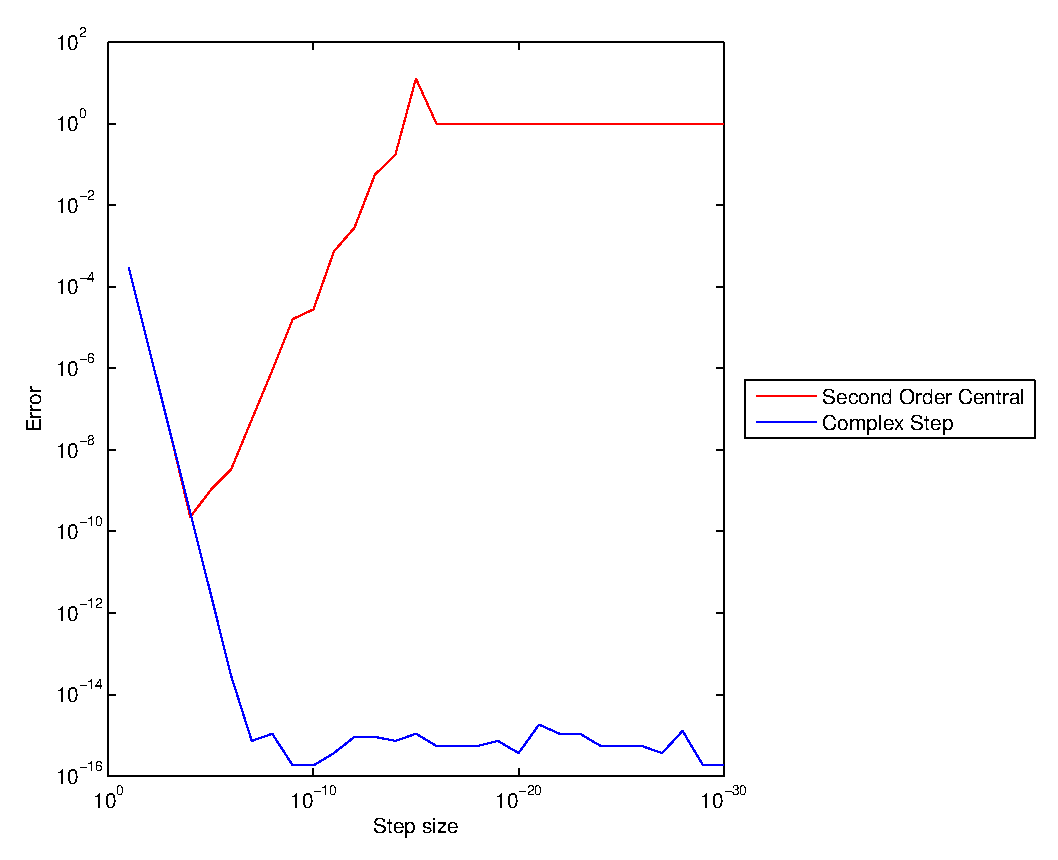
\includegraphics[scale = 0.7]{DerivativeError.eps}
			\caption{Error comparison between the complex step and second order central methods of differentiation}\label{fig:DerErr}
		\end{figure}
		From this, the optimal step size was found to be $1.0\times 10^{-5}$.
		
		The gradient of the drag coefficient with a wing reference area of 20 and an aspect ratio of 10 comes out to be
		\begin{eqnarray*}
			\nabla C_{D_{CS}} &=& \left\langle \textcolor{blue}{-0.0001478637086}2224425, \textcolor{blue}{-0.000717943586}27084835 \right\rangle \\
			\nabla C_{D_{FD}} &=& \left\langle \textcolor{blue}{-0.0001478637086}5563225, \textcolor{blue}{-0.000717943586}30014599 \right\rangle
		\end{eqnarray*}

	\section{Now For the Fun Stuff}
	
		First, note that I used the version of the wing code that had $I_z = (\pi/4)[r^3 - (r-t)^3]$. The first two parts of
		this section are not very difficult to implement but, as expected, are slow. I again when with a second order central difference method
		for the finite difference computations. This method requires that for each derivative with respect to a different input variable, two 
		function evaluations are needed. Since we wanted derivatives with respect to each tube diameter this meant that 12 function evaluations
		were needed. With the first two function evaluations, both $\frac{\partial\gamma_{tip}}{\partial D_1}$ and $\frac{\partial u_j}{\partial D_1}$
		can be computed. After that 10 more function calls are required to compute the last 5 derivatives we are interested in.
		
		This is obviously less than ideal for a number of reasons. If the derivatives of interested are being computed from a function that 
		takes an appreciable amount of time to compute, calling this function more that once is not advisable. Another other issue is if a
		large number of derivatives are desired, this method requires twice the amount of function calls as there are derivatives. If 
		both of these issues are present at once, which they commonly are, the finite difference method becomes nonstarter. To make matters 
		worse is the fact that finite difference methods are subject to subtractive cancellation, causing even more error if an appropriate 
		step size is not chosen. The topping on the crappy derivative cake is that, for a central difference scheme, an extra function
		evaluation is needed to get the actual value of the function at the point of interest!
		
		Next up is the complex step method. On the surface this approach looks better than the last. It only requires a single function call
		per derivative of interest. It is also far more accurate than any finite difference method can be. To top it off, no extra function
		call is needed to get the value of the function at the point of interest. The devil, however, is in the details. Complex numbers are
		effectively a grouping of two individual numbers. This means that every line that has a complex number in it now needs twice the
		operations to compute. This can drastically reduce the speed of this method bringing it on par with the finite difference method in
		terms of computation time. It still has advantages over finite differences, the biggest being the accuracy, but it is also, generally,
		much easier to implement.
		
		The direct and adjoint analytic methods are more difficult to implement but have a greater payoff. These methods work by directly
		modifying the function of interest to compute the derivatives of interest accurately and fast.
		
		The direct method takes the form
		\begin{eqnarray}
			\frac{\mathrm{d}f}{\mathrm{d}x} &=& \frac{\partial F}{\partial x} + \frac{\partial F}{\partial y}\frac{\mathrm{d}y}{\mathrm{d}x} \\
			-\frac{\partial R}{\partial y}\frac{\mathrm{d}y}{\mathrm{d}x} &=& \frac{\partial R}{\partial x}
		\end{eqnarray}
		The residual equation in this problem is
		\begin{equation}
			K_{kj}u_j - F = 0
		\end{equation}
		Where $K_ki$ is the stiffness matrix, $u_i$ is the vector of element displacements, and $F$ is a vector of applied forces, not the
		functions of interest.
		
		The since the input variables we are interested in are the tube diameters, we can write the following.
		\begin{equation}
			\frac{\partial R}{\partial x} = \frac{\partial R_k}{\partial D_i} = \frac{\partial (K_{kj}u_j - F)}{\partial D_i} = \frac{\partial K_{kj}}{\partial D_i}u_j
		\end{equation}
		$F$ does not directly depend on $D_i$ so it drops out of the equation. Similarly $u_j$ has no explicit dependance on $D_i$ so it is
		treated like a constant. This is the most complicated term as will be seen. It expands out to the following.
		\begin{equation}
			\frac{\partial K_{kj}}{\partial D_i}u_j = \begin{bmatrix} \frac{\partial K_{1,1}}{\partial D_1} & \dots & \frac{\partial K_{1,1}}{\partial D_6} \\
 												                     \frac{\partial K_{2,1}}{\partial D_1} & \dots & \frac{\partial K_{2,1}}{\partial D_6} \\
 												                     \vdots & \ddots & \vdots \\
 												                     \frac{\partial K_{12,1}}{\partial D_1} & \dots & \frac{\partial K_{12,1}}{\partial D_6} \end{bmatrix}u_1
 												                     + \dots + 
 												     \begin{bmatrix} \frac{\partial K_{1,12}}{\partial D_1} & \dots & \frac{\partial K_{1,12}}{\partial D_6} \\
 												                     \frac{\partial K_{2,12}}{\partial D_1} & \dots & \frac{\partial K_{2,12}}{\partial D_6} \\
 												                     \vdots & \ddots & \vdots \\
 												                     \frac{\partial K_{12,12}}{\partial D_1} & \dots & \frac{\partial K_{12,12}}{\partial D_6} \end{bmatrix}u_{12}
		\end{equation}
		To build this matrix each variable of interest is perturbed, using complex steps in this case, the stiffness matrix is built and
		the derivatives are stored till after the displacements are computed. Once the displacements are found, they are multiplied in,
		and each matrix is summed to get a single 12x6 matrix.

		The next residual term is much simpler than the last. Using the same residual equation, it expands to the following.
		\begin{equation}
			\frac{\partial R}{\partial y} = \frac{\partial R_k}{\partial u_j} = \frac{\partial (K_{kj}u_j - F)}{\partial u_j} = K_{kj}
		\end{equation}
		This convenient solution means no extra work needs to be done to obtain this term.
		
		The partial derivatives of the function of interest are also easy to come by. The derivative with respect to the input variables
		is the easiest to compute.
		\begin{equation}
			\frac{\partial F}{\partial x} = \frac{\partial \gamma_{tip}}{\partial D_i} = 0
		\end{equation}
		We get this solution because the twist of the wing has no explicit dependance on the diameter of the spar tubes.
		
		The last set of partial derivatives need is the following
		\begin{equation}
			\frac{\partial F}{\partial y} = \frac{\partial \gamma_{tip}}{\partial u_j}
		\end{equation}
		This is still very simple to compute and does not require recomputing the entire solution. To get the total derivative of the
		tip twist angle with respect to each of the spar diameters we end up with this final expression.
		\begin{equation}
			\frac{\mathrm{d}f}{\mathrm{d}x} = -\frac{\partial \gamma_{tip}}{\partial u_j}K_{kj}^{-1}\frac{\partial K_{kj}}{\partial D_i}u_j
		\end{equation}

		To compute the derivative of the displacements with respect to $D_1$ the same process can be followed. However, upon inspection
		we can see that we have already computed the total derivative with respect to all the input variables as a part of the previous
		solution.
		\begin{equation}
			\frac{\mathrm{d}y}{\mathrm{d}x} = -\frac{\partial R}{\partial y}^{-1}\frac{\partial R}{\partial x} = -K_{kj}^{-1}\frac{\partial K_{kj}}{\partial D_i}u_j
		\end{equation}
		So without doing any extra computations we have all the derivatives of interest.
		
		This method is much more difficult to implement but the tradeoff is an accurate derivative computed quickly. It avoids running
		the bulk of the code multiple times, unlike finite differences or the complex step, and still achieves good accuracy.
		
		The adjoint method is slightly different, but does share some of the same terms. It takes the form
		\begin{eqnarray}
			\frac{\mathrm{d}f}{\mathrm{d}x} &=& \frac{\partial F}{\partial x} + \frac{\mathrm{d}f}{\mathrm{d}r}\frac{\partial R}{\partial x} \\
			-\frac{\partial R}{\partial y}^T\frac{\mathrm{d}f}{\mathrm{d}r}^T &=& \frac{\partial F}{\partial y}^T
		\end{eqnarray}
		also written as
		\begin{eqnarray}
			\frac{\mathrm{d}f}{\mathrm{d}x} &=& \frac{\partial F}{\partial x} + \psi_{k}\frac{\partial R}{\partial x} \\
			-\frac{\partial R}{\partial y}^T\psi_{k}^T &=& \frac{\partial F}{\partial y}^T
		\end{eqnarray}
		
		The $\frac{\partial F}{\partial x}$, $\frac{\partial R}{\partial x}$, $\frac{\partial R}{\partial y}$, and $\frac{\partial F}{\partial y}$
		terms all remain the same as the direct method, they are just applied differently.
		\begin{equation}
			\frac{\mathrm{d}f}{\mathrm{d}x} = -K_{kj}^{-1}\frac{\partial \gamma_{tip}}{\partial u_j}\frac{\partial K_{kj}}{\partial D_i}u_j
		\end{equation}

		Getting the displacement derivatives isn't quite as straight forward as it is with the direct approach. If we follow the same
		derivation for these derivatives we get the following.
		\begin{equation}
			\psi_{k}^T = -{\frac{\partial R}{\partial y}^T}^{-1}\frac{\partial F}{\partial y}^T = 
				-{\frac{\partial (K_{kj}u_j - F)}{\partial u_j}^T}^{-1}\frac{\partial u_j}{\partial u_j}^T = -{K_{kj}^{T}}^{-1}I^T
		\end{equation}
		Once this is computed it is multiplied by the first column of the $\frac{\partial R}{\partial x}$ matrix that was computed earlier.
		
		Both the adjoint and direct analytic methods are ideal ways to compute many derivatives of computationally expensive functions.
		They avoid running re-computing the residual functions more than once that are often very computationally heavy. They also produce
		very accurate results. The drawback of this method is the implementation. They are both more difficult to implement than
		either the complex step or finite difference method and require direct modifications to the code. If source code is not
		available than these methods are no-goes.
		
		To compare some actual numbers from these methods the table below lists the derivative values for $\frac{\partial \gamma_{tip}}{\partial D_1}$
		as well as the average relative computation time with respect to the complex step method.
		\begin{center}
			\begin{tabular}{| p{4cm} | c | c |}
				\hline
				Method & $\frac{\partial \gamma_{tip}}{\partial D_1}$ & Relative Computation time \\ \noalign{\hrule height 2pt}
				Complex Step 		& \textcolor{blue}{25.3876039545}9745922153 & 1.00000 \\ \hline
				Direct Analytic 		& \textcolor{blue}{25.38760395458}740504182 & 0.84208 \\ \hline
				Direct Analytic 		& \textcolor{blue}{25.38760395458}931640178 & 0.80878 \\ \hline
				Finite Difference 	& \textcolor{blue}{25.38760}420600638667565 & 1.17097 \\ \hline
			\end{tabular}
		\end{center}
		This comparison makes the benefits of analytic methods clear.

		The full results of the derivatives are listed below. They are listed as column vectors for convenience.
		
		\textbf{Complex Step:}
		\begin{equation}
			\frac{\partial \gamma_{tip}}{\partial D_i} = \begin{bmatrix}    25.3876039545975 \\
												   190.5337701576488 \\
												   139.1626613182595 \\
												   16.8047861692089 \\
												   52.7252871310561 \\
												   20.1297866329028
   			\end{bmatrix}
		\end{equation}

		\begin{equation}
			\frac{\partial u_j}{\partial D_1} = \begin{bmatrix} 0 \\	0\\ 0\\	-1.31510632884564 \\	0.202534736589733 \\	-0.397311904736405 \\	-3.55401169488538 \\	0.180896840526585 \\	-0.441672542746385 \\	0 \\	0 \\	0 \\	-1.70740304599702 \\	0.520845898385775 \\	-0.0544778498517718 \\	-3.98608999725024 \\	0.291399533050542 \\	-0.443705665383865 \\
   			\end{bmatrix}
		\end{equation}
		
		
		
		\pagebreak
		\textbf{Direct Analytic:}
		\begin{equation}
			\frac{\partial \gamma_{tip}}{\partial D_i} = \begin{bmatrix}    25.3876039545874 \\
   190.5337701576020 \\
   139.1626613174258 \\
   16.8047861693346 \\
   52.7252871319023 \\
   20.1297866339990
   			\end{bmatrix}
		\end{equation}

		\begin{equation}
			\frac{\partial u_j}{\partial D_1} = \begin{bmatrix} 0 \\
                   0 \\
                   0 \\
  -1.315106328846540 \\
   0.202534736590065 \\
  -0.397311904736402 \\
  -3.554011694887727 \\
   0.180896840527013 \\
  -0.441672542746213 \\
                   0 \\
                   0 \\
                   0 \\
  -1.707403045997769 \\
   0.520845898386072 \\
  -0.054477849851675 \\
  -3.986089997252424 \\
   0.291399533050952 \\
  -0.443705665383688
   			\end{bmatrix}
		\end{equation}
		
		
		\pagebreak
		\textbf{Adjoint Analytic:}
		\begin{equation}
			\frac{\partial \gamma_{tip}}{\partial D_i} = \begin{bmatrix} 25.3876039545893 \\
   190.5337701576048 \\
   139.1626613174270 \\
   16.8047861693346 \\
   52.7252871319019 \\
   20.1297866339992
   			\end{bmatrix}
		\end{equation}

		\begin{equation}
			\frac{\partial u_j}{\partial D_1} = \begin{bmatrix} 0 \\
                   0 \\
                   0 \\ 
  -1.315106328846539 \\
   0.202534736590062 \\
  -0.397311904736405 \\
  -3.554011694887722 \\
   0.180896840526991 \\
  -0.441672542746246 \\
                   0 \\
                   0 \\
                   0 \\
  -1.707403045997777 \\
   0.520845898386073 \\
  -0.054477849851679 \\
  -3.986089997252454 \\
   0.291399533050944 \\
  -0.443705665383720
   			\end{bmatrix}
		\end{equation}
		
		
		\pagebreak
		\textbf{Second Order Central Finite Difference:}
		\begin{equation}
			\frac{\partial \gamma_{tip}}{\partial D_i} = \begin{bmatrix} 25.3876042060064 \\
   190.5337703194121 \\
   139.1626614757335 \\ 
   16.8047860635845 \\
   52.7252869604311 \\
   20.1297866877503
   			\end{bmatrix}
		\end{equation}

		\begin{equation}
			\frac{\partial u_j}{\partial D_1} = \begin{bmatrix} 0 \\
                   0 \\
                   0 \\
  -1.315106329266569 \\ 
   0.202534736520182 \\
  -0.397311905066949 \\
  -3.554011696826898 \\
   0.180896837881535 \\
  -0.441672547119021 \\
                   0 \\
                   0 \\
                   0 \\
  -1.707403047501721 \\
   0.520845898754202 \\
  -0.054477850411350 \\
  -3.986090003460507 \\
   0.291399532474299 \\
  -0.443705669872507
   			\end{bmatrix}
		\end{equation}
\end{document}
